\section{Tournament Analysis}

\subsection{Pairwise Games}
For both configurations chosen by Kevin for pairwise tournaments, we were the dominant player and \textbf{won every single matchup}, even when ran again in independent simulations. We believe that this is because we were the only group to adopt a strategy with outwardly aggressive elements, as described in the Border Strategy section. In pairwise competition, aggressive behavior doesn’t benefit a third player, which can make it a viable strategy if it sufficiently disrupts the enemy player. The following screenshots, taken in simulations running the pairwise n=2, d=2, t=10 configuration show how an aggressive border strategy was able to disrupt enemy players g1, g3, g6, g7, and g8 (not pictured), in the early to mid stages of the game to allow our player to claim significantly more space before the game entered later stages:\\
\begin{figure}[h]
\center
\includegraphics[scale=0.3]{tourn1.png}
\caption{}
\label{fig:tourn1}
\end{figure}

\begin{figure}[h]
\center
\includegraphics[scale=0.3]{tourn2.png}
\caption{}
\label{fig:tourn2}
\end{figure}

\begin{figure}[h]
\center
\includegraphics[scale=0.3]{tourn3.png}
\caption{}
\label{fig:tourn3}
\end{figure}

\begin{figure}[h]
\center
\includegraphics[scale=0.3]{tourn4.png}
\caption{}
\label{fig:tourn4}
\end{figure}
\clearpage
The aggressive strategy was also useful when trying to quell enemy infiltrations into our clusters, as in one simulation against g4:\\
\begin{figure}[h]
\center
\includegraphics[scale=0.3]{tourn5.png}
\caption{}
\label{fig:tourn5}
\end{figure}

\begin{figure}[h]
\center
\includegraphics[scale=0.3]{tourn6.png}
\caption{}
\label{fig:tourn6}
\end{figure}




The grouping of blue g4 cells in the friendly cluster pictured above was inhibited from growing and disrupting the reproduction within our cluster because several cells were designated as attackers to prevent it from growing.\\
There were also cases in the pairwise competition—such as with g2—where we were losing in the mid-game, but eventually overtook the other player because of our late-game random player strategy which efficiently packed cells into space that we claimed in the early game:\\
\begin{figure}[h]
\center
\includegraphics[scale=0.3]{tourn7.png}
\caption{}
\label{fig:tourn7}
\end{figure}

\begin{figure}[h]
\center
\includegraphics[scale=0.3]{tourn8.png}
\caption{}
\label{fig:tourn8}
\end{figure}
Similar phenomena were observed for the n=1, d=5, t=20 configuration, which produced wins with even larger margins!\\


All in all, the mean margin of victory for the n=2, d=2, t=10 configuration was 1147.5, and for the n=1, d=5, t=20 configuration it was 1254. These means were skewed by outlier results, so we also calculated the median margins of victory which were 872 and 1245.5 respectively.\\

\subsection{All Player Games}
Our expectation for Slather was that since our group strategy relies on creating and expanding a large cluster, we would perform poorly when we could not create as large a cluster. This would happen either if there were too many players or too many starting cells, which would lead to smaller clusters. We came in fifth for most of the n=63, d=2, t=10 games. Unexpectedly, we performed better than we expected for n = 20, coming in the top four places for most of the games. 
We performed very well for the games with n = 1, d=1 and t =2 coming in first three times and in the top 3 in six out of ten games. We also performed well in n=1,d=4,t=4 coming in the top three for about half of the games. This was expected since low n values meant that we would form a single large cluster.
We did not perform as well as we hoped for the case n=1,d=10,t=1, coming in fifth for a majority of the games. We suspect that other players used the increased vision better than we did.
We infer from these runs that our player outperforms the others for the case that n is small, and there is low vision, irrespective of pheromones, but does poorly in games with large vision range or large number of starting cells.
During our tests, we concluded that the choice of parameters is very important and determines the performance for different cases. We were able to determine a good choice of parameters for 2-player games and for multi player games separately, but we were unable to unify the two. 
Below is the result of tuning our parameters to play well against multiple players.\\

\begin{figure}[h]
\center
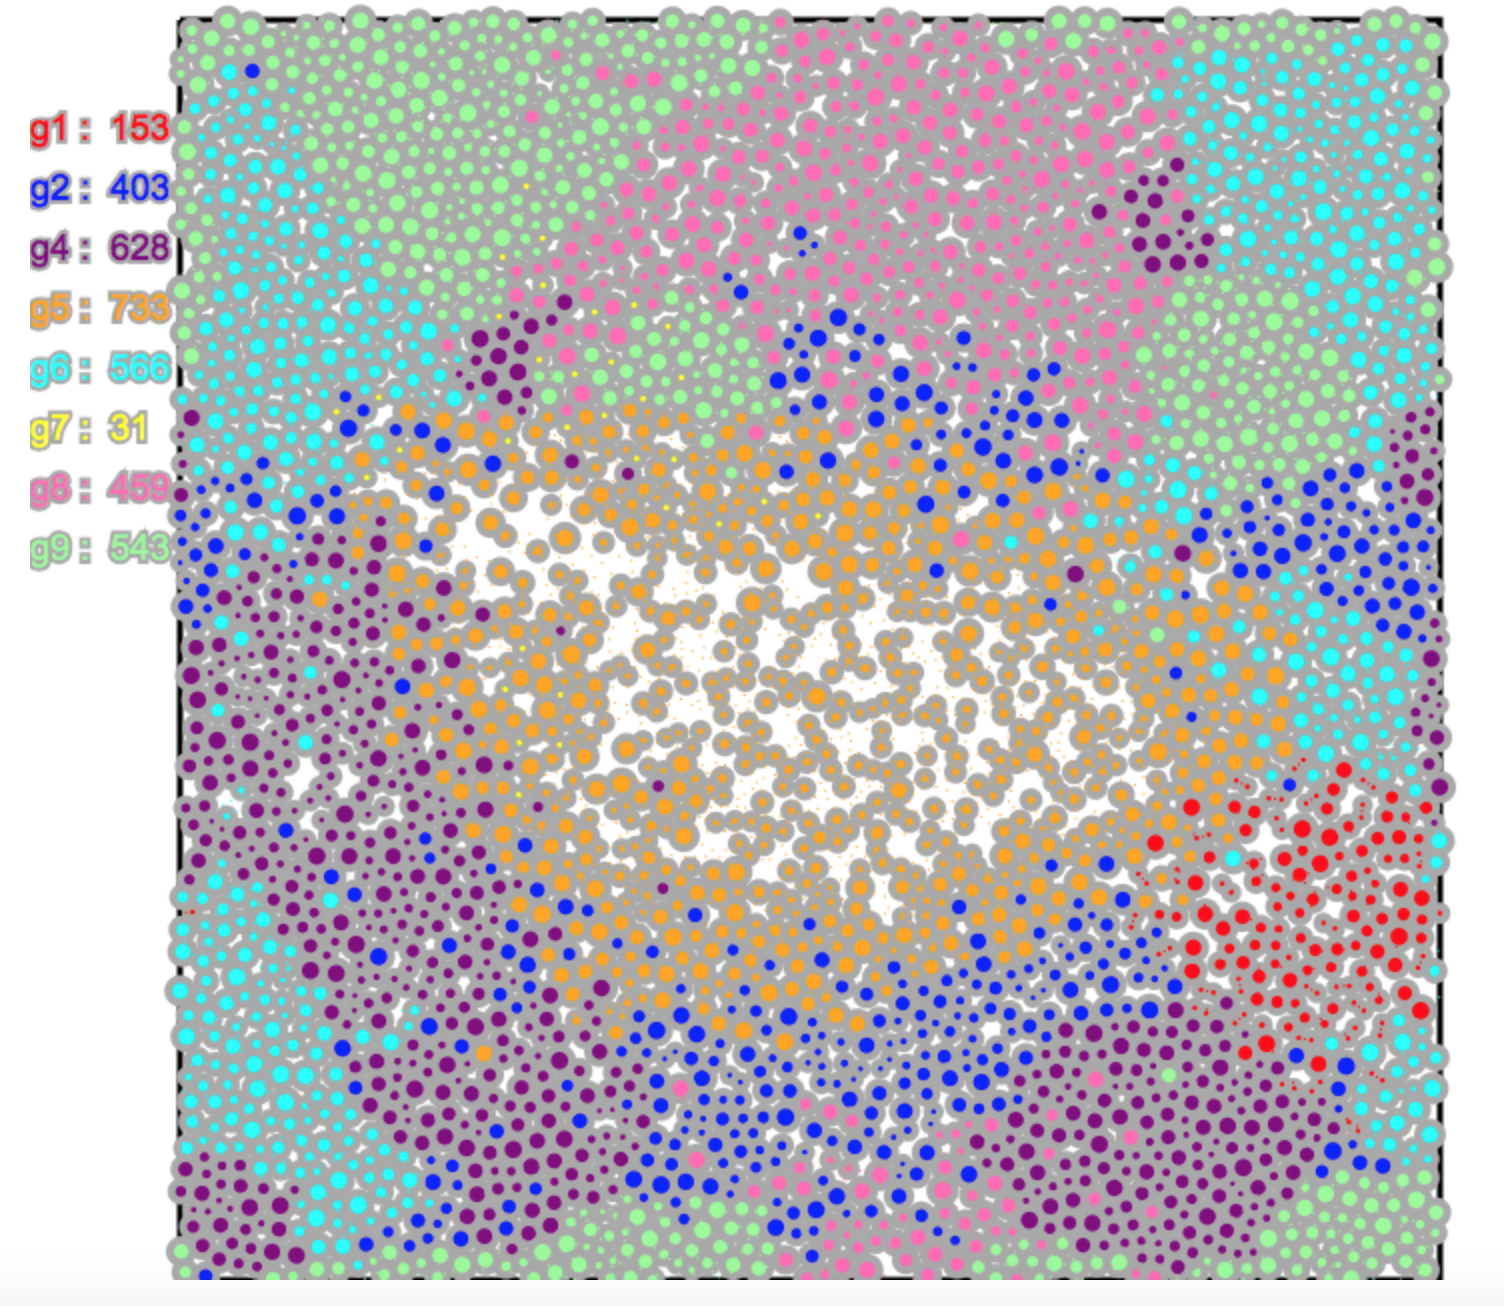
\includegraphics[scale=0.6]{multi.png}
\caption{}
\label{fig:multi}
\end{figure}